



%\tikzset{every picture/.style={line width=0.75pt}} %set default line width to 0.75pt        

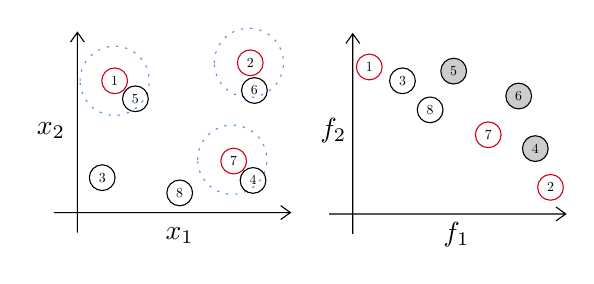
\begin{tikzpicture}[x=0.5pt,y=0.5pt,yscale=-1,xscale=1]
%uncomment if require: \path (0,300); %set diagram left start at 0, and has height of 300

%Shape: Circle [id:dp5136866411017809] 
\draw  [color={rgb, 255:red, 74; green, 144; blue, 226 }  ,draw opacity=1 ][dash pattern={on 0.84pt off 2.51pt}] (69,105) .. controls (69,91.19) and (80.19,80) .. (94,80) .. controls (107.81,80) and (119,91.19) .. (119,105) .. controls (119,118.81) and (107.81,130) .. (94,130) .. controls (80.19,130) and (69,118.81) .. (69,105) -- cycle ;
%Shape: Circle [id:dp3061612047883613] 
\draw  [color={rgb, 255:red, 74; green, 144; blue, 226 }  ,draw opacity=1 ][dash pattern={on 0.84pt off 2.51pt}] (166,92) .. controls (166,78.19) and (177.19,67) .. (191,67) .. controls (204.81,67) and (216,78.19) .. (216,92) .. controls (216,105.81) and (204.81,117) .. (191,117) .. controls (177.19,117) and (166,105.81) .. (166,92) -- cycle ;
%Shape: Axis 2D [id:dp3645341276574614] 
\draw  (50,200.22) -- (221,200.22)(67.1,70) -- (67.1,214.69) (214,195.22) -- (221,200.22) -- (214,205.22) (62.1,77) -- (67.1,70) -- (72.1,77)  ;
%Shape: Circle [id:dp595877391054507] 
\draw  [color={rgb, 255:red, 74; green, 144; blue, 226 }  ,draw opacity=1 ][dash pattern={on 0.84pt off 2.51pt}] (154,162) .. controls (154,148.19) and (165.19,137) .. (179,137) .. controls (192.81,137) and (204,148.19) .. (204,162) .. controls (204,175.81) and (192.81,187) .. (179,187) .. controls (165.19,187) and (154,175.81) .. (154,162) -- cycle ;
%Shape: Axis 2D [id:dp14963900792703488] 
\draw  (249,201.22) -- (420,201.22)(266.1,71) -- (266.1,215.69) (413,196.22) -- (420,201.22) -- (413,206.22) (261.1,78) -- (266.1,71) -- (271.1,78)  ;

% Text Node
\draw  [color={rgb, 255:red, 208; green, 2; blue, 27 }  ,draw opacity=1 ]  (94, 105) circle [x radius= 9.3, y radius= 9.3]   ;
\draw (94,105) node [scale=0.5] [align=left] {1};
% Text Node
\draw  [color={rgb, 255:red, 0; green, 0; blue, 0 }  ,draw opacity=1 ]  (109, 118) circle [x radius= 9.3, y radius= 9.3]   ;
\draw (109,118) node [scale=0.5] [align=left] {5};
% Text Node
\draw  [color={rgb, 255:red, 208; green, 2; blue, 27 }  ,draw opacity=1 ]  (192, 92) circle [x radius= 9.3, y radius= 9.3]   ;
\draw (192,92) node [scale=0.5] [align=left] {2};
% Text Node
\draw    (195, 112) circle [x radius= 9.3, y radius= 9.3]   ;
\draw (195,112) node [scale=0.5] [align=left] {6};
% Text Node
\draw  [color={rgb, 255:red, 208; green, 2; blue, 27 }  ,draw opacity=1 ]  (180, 163) circle [x radius= 9.3, y radius= 9.3]   ;
\draw (180,163) node [scale=0.5] [align=left] {7};
% Text Node
\draw    (194, 177) circle [x radius= 9.3, y radius= 9.3]   ;
\draw (194,177) node [scale=0.5] [align=left] {4};
% Text Node
\draw    (141, 186) circle [x radius= 9.3, y radius= 9.3]   ;
\draw (141,186) node [scale=0.5] [align=left] {8};
% Text Node
\draw    (85, 175) circle [x radius= 9.3, y radius= 9.3]   ;
\draw (85,175) node [scale=0.5] [align=left] {3};
% Text Node
\draw  [color={rgb, 255:red, 208; green, 2; blue, 27 }  ,draw opacity=1 ]  (278, 95) circle [x radius= 9.3, y radius= 9.3]   ;
\draw (278,95) node [scale=0.5] [align=left] {1};
% Text Node
\draw  [color={rgb, 255:red, 0; green, 0; blue, 0 }  ,draw opacity=1 ][fill={rgb, 255:red, 0; green, 0; blue, 0 }  ,fill opacity=0.2 ]  (339, 98) circle [x radius= 9.3, y radius= 9.3]   ;
\draw (339,98) node [scale=0.5] [align=left] {5};
% Text Node
\draw  [color={rgb, 255:red, 208; green, 2; blue, 27 }  ,draw opacity=1 ]  (409, 182) circle [x radius= 9.3, y radius= 9.3]   ;
\draw (409,182) node [scale=0.5] [align=left] {2};
% Text Node
\draw  [fill={rgb, 255:red, 0; green, 0; blue, 0 }  ,fill opacity=0.2 ]  (386, 116) circle [x radius= 9.3, y radius= 9.3]   ;
\draw (386,116) node [scale=0.5] [align=left] {6};
% Text Node
\draw  [color={rgb, 255:red, 208; green, 2; blue, 27 }  ,draw opacity=1 ]  (364, 144) circle [x radius= 9.3, y radius= 9.3]   ;
\draw (364,144) node [scale=0.5] [align=left] {7};
% Text Node
\draw  [fill={rgb, 255:red, 0; green, 0; blue, 0 }  ,fill opacity=0.2 ]  (398, 154) circle [x radius= 9.3, y radius= 9.3]   ;
\draw (398,154) node [scale=0.5] [align=left] {4};
% Text Node
\draw    (322, 126) circle [x radius= 9.3, y radius= 9.3]   ;
\draw (322,126) node [scale=0.5] [align=left] {8};
% Text Node
\draw    (302, 105) circle [x radius= 9.3, y radius= 9.3]   ;
\draw (302,105) node [scale=0.5] [align=left] {3};
% Text Node
\draw (141,217) node   {$x_{1}$};
% Text Node
\draw (48,141) node   {$x_{2}$};
% Text Node
\draw (341,216) node   {$f_{1}$};
% Text Node
\draw (252,141) node   {$f_{2}$};


\end{tikzpicture}

